\section{Message Board}
\Writetofile{hints}{\protect\section{Message Board 12}}
\Writetofile{soln}{\protect\newpage\protect\section{Message Board 12}}

\subsection{Problem 1}
Given a circle and a line that does not intersect the circle, construct the inverse of the line with respect to the circle.

\begin{mdsoln}
In case we are not given the center $O$ of the given circle, we can construct it by picking three distinct points of the circle and finding the circumcenter of the triangle they form.

Let $P$ be the foot of the altitude from $O$ to the given line $\ell$. We know that $\ell$ maps to a circle $\omega$ through $O$. By symmetry, $\omega$ must have diameter $OP'$, where $P'$ is the inverse of $P$. We construct $P'$ as described in class, by drawing a tangent $PX$ to the given circle (where $X$ is on the given circle) and finding the foot of the altitude from $X$ to the segment $OP$.

Having located $P'$, it is simple to construct $\omega$ as the circle with diameter $OP'$.
    
\end{mdsoln}

\subsection{Problem 2}
Given a circle and a line that intersects the circle in two non-diametrically opposed points, prove that the inverse of the line with respect to the circle is a circle. Prove that if the line is tangent to the circle, the image of the line is still a circle. (We want the details of the proof that the inverses of the lines described are circles - don't just say 'the inverse of a line not through the center of inversion is a circle')

\begin{mdsoln}    
Let $\omega$ be the circle, with center $O$. Let $\ell$ be the line, and consider first the case where $\ell$ intersects $\omega$ in two distinct points $A$ and $B$.

Let $P$ be on $\ell$ (and distinct from $A$ and $B$). Let $P'$ be the inverse of $P$. Observe that since $(OP)(OP')=OA^2=OB^2$, we must have $\triangle OAP\sim \triangle OP'A$ and $\triangle OBP\sim \triangle OP'B$.

Consider first the case where $P$ is on segment $AB$. Then, $\angle P'AO+\angle OBP'=\angle OPA+\angle BPO=180^\circ$, so $P'$ lies on the circumcircle of $\triangle OAB$.

Now suppose $P$ is not on segment $AB$. Then, $\angle OAP'=\angle APO=\angle BPO=\angle OBP'$, so in this case also $P'$ must lie on the (fixed) circumcircle of $\triangle OAB$.

Clearly, $O$ is in the inverse of $\ell$ since the point at infinity (which is on $\ell$) maps to $O$. Now consider a point $Q$ on $\omega_1$ distinct from $O$. Ray $OQ$ must intersect $\ell$ at some point $Q'$. Then, our argument above shows that the inverse of $Q'$ must be a point on $OQ$ that is also on $\omega_1$ - this point, since it is clearly not $O$, must be $Q$, showing that all points on $\omega_1$ are the images of points on $\ell$ and completing the proof that $\omega_1$ is the image of $\ell$ under inversion about $\omega$.

Now suppose that $\ell$ is tangent to $\omega$ at some point $A$. Pick some point $P$ on $\ell$ with inverse $P'$. Since $(OP)(OP')=OA^2$, we must have $\triangle OAP\sim \triangle OP'A$. Hence, $\angle AP'O$ is a right angle, so $P'$ must be on the circle $\omega_2$ with diameter $OA$.

Conversely, if $Q$ is any point of $\omega_2$, we can use our previous argument to show that $Q$ is the image of a point on $\ell$. We conclude that $\ell$ maps to $\omega_2$.
\end{mdsoln}

\subsection{Problem 3}
Find a quick proof of Ptolemy’s Inequality using one of the facts about inversion we learned in class. (Reminder: Ptolemy’s Inequality states that if $A, B, C, D$ are points in a plane, then $AB \cdot CD + AD\cdot BC \geq AC\cdot BD$, with equality if and only if the four points are concyclic.)

\textit{Has hints.}
\begin{sketch}
    \begin{enumerate}
        \item Invert with respect to A with an arbitrary radius.
        \item Use the result of problem 2 on the final.
    \end{enumerate}
\end{sketch}

\begin{mdsoln}
Invert with respect to a circle centered at $A$ of arbitrary radius $r$, so that $B,C,D$ go to $B',C',D'$, respectively. Then, by the Triangle Inequality, $C'D'+B'C'\ge B'D'$. Equality occurs if and only if $B',C',D'$ are collinear in that order, which happens if and only if $ABCD$ is a convex cyclic quadrilateral (or $B,C,D$ lie in that order on a line passing through $A$, which might be seen as a limiting case of $ABCD$ cyclic with an infinitely large circumcircle).

Observe that $AB=r^2/AB'$, $AC=r^2/AC'$, and $AD=r^2/AD'$. Using the formula from 2b on the Final Challenge Set (relating distances after inversion to distances before), we find that since $BC$ is the image of $B'C'$ under an inversion about a circle of radius $r$ centered at $A$,$$BC=\frac{r^2(B'C')}{(AB')(AC')}$$and similar expressions for $B'D'$ and $C'D'$. Hence,\begin{eqnarray*}AB\cdot CD+AD\cdot BC&=&\frac{r^2}{AB'}\cdot \frac{r^2(C'D')}{(AC')(AD')}+\frac{r^2}{AD'}\cdot \frac{r^2(B'C')}{(AB')(AC')}\\ &=&\frac{r^4}{(AB')(AC')(AD')}(C'D'+B'C')\\ &\ge &\frac{r^4}{(AB')(AC')(AD')}(B'D')\\ &=&\frac{r^2}{AC'}\cdot \frac{r^2(B'D')}{(AB')(AD')}\\ &=&AC\cdot BD\end{eqnarray*}with equality if and only if $ABCD$ is cyclic.    
\end{mdsoln}

\subsection{Problem 4}
Circles $A$, $B$, and $C$ all pass through point $X$. The radical axis of circles $A$ and $B$ passes through the center of $C$; the radical axis of circles $B$ and $C$ passes through the center of $A$. Prove that the radical axis of $A$ and $C$ passes through the center of $B$.

% https://s3.amazonaws.com/classroom.artofproblemsolving.com/Classes/GeomOlympiad/Images/threerads.gif
\begin{center}
    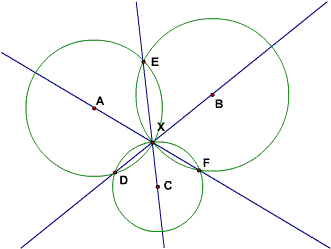
\includegraphics[scale=0.6]{threerads}
\end{center}

\begin{mdsoln}
Invert about a circle of arbitrary radius centered at the point $X$. Circles $A,B,C$ invert to lines $\ell_A,\ell_B,\ell_C$, respectively. Let $\ell_A$ and $\ell_B$ meet at $C_1$. Define $A_1$ and $B_1$ similarly. Let $m_A$ be the radical axis of circles $B$ and $C$. Define $m_B$ and $m_C$ similarly. Clearly, $m_A$, $m_B$, and $m_C$ invert to themselves, since they all pass through $X$. Then, note that $m_A$ must in fact be the line $A_1X$; likewise, $m_B$ and $m_C$ are $B_1X$ and $C_1X$ respectively. Since $m_C$ passes through the center of $C$, it is perpendicular to circle $C$ and so must be perpendicular to $\ell_C$. Then, $C_1X\perp A_1B_1$. Likewise, since $m_A$ passes through the center of $A$, $A_1X\perp B_1C_1$. Hence, $X$ must be the orthocenter of $\triangle A_1B_1C_1$. Therefore, $B_1X\perp A_1C_1$, implying that $m_B\perp \ell_B$. Therefore, $m_B$ must be perpendicular to circle $B$ and so must pass through its center, as desired.    
\end{mdsoln}

\subsection{Problem 5}
We are given four points $A$, $B$, $C$, and $D$ such that no 3 are collinear. Prove that the angle between the circles circumscribed about triangles $ABC$ and $BCD$ is equal to the angle between the circles circumscribed about the triangles $CDA$ and $DAB$.

% https://s3.amazonaws.com/classroom.artofproblemsolving.com/Classes/GeomOlympiad/Images/circangl.gif
\begin{center}
    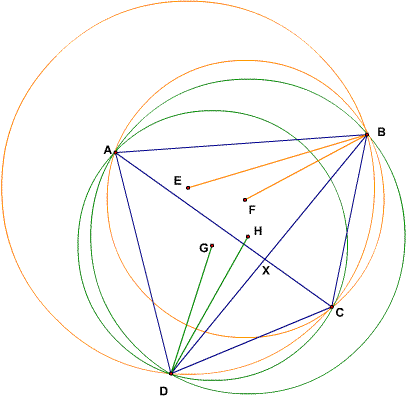
\includegraphics[scale=0.6]{circangl}
\end{center}
\begin{mdsoln}
Let $\omega_A,\omega_B,\omega_C,\omega_D$ be the circumcircles of $\triangle BCD,\triangle CDA,\triangle DAB,\triangle ABC$, respectively. We invert about $B$, so that points $A,C,D$ invert to $A',C',D'$, respectively. Circles $\omega_D$ and $\omega_A$ invert to lines $A'C'$ and $D'C'$, respectively. Hence, the angle between $\omega_D$ and $\omega_A$ is equal to$$\angle A'C'D'=|\angle A'C'B -\angle D'C'B|=|\angle BAC-\angle BDC|$$
Likewise, we can conclude that the angle between $\omega_B$ and $\omega_C$ equals $|\angle DCA-\angle DBA|$. But $\angle BAC-\angle BDC=\angle DCA-\angle DBA$, since$$\angle BAC+\angle DBA=180^\circ-\angle AXB=180^\circ-\angle CXD=\angle DCA+\angle BDC$$We conclude that $|\angle BAC-\angle BDC|=|\angle DCA-\angle DBA|$, proving the problem.    
\end{mdsoln}

\subsection{Problem 6}
Given a point $A$ and two circles $k_1$ and $k_2$, construct a third circle $k_3$ so that $k_3$ passes through $A$ and is tangent to $k_1$ and $k_2$.

\begin{mdsoln}
In this proof we assume that it is possible to construct the inverse of a given circle or line about a given circle. We know that we can invert a point (by the method discussed in class). To invert a circle or line that maps to a circle, it suffices to invert 3 distinct points and draw the circumcircle of the inverses; to invert a circle or line that maps to a line, we may invert 2 distinct points and draw the line through the inverses.

In this problem, we will invert everything about a circle centered at $A$ and of arbitrary radius. Let figures $j_1$ and $j_2$ (either lines or circles) be the inverses of $k_1$ and $k_2$, respectively. Any circle $k_3$ of the desired form must invert to a line $j_3$ not passing through $A$, such that $j_3$ is parallel to $j_1$ if $j_1$ is a line and is tangent to $j_1$ if $j_1$ is a circle, and similarly with $j_2$. Conversely, any line $j_3$ satisfying these conditions must invert to a circle $k_3$ of the desired form.

Case 1: $A$ lies on both $k_1$ and $k_2$.
Then, $j_1$ and $j_2$ must be lines. Any line $j_3$, if it exists, must be parallel to both of them. Therefore, $j_1$ must be parallel to $j_2$ if $j_3$ and hence $k_3$ is to exist. This means that there is no $k_3$ possible if $k_1$ and $k_2$ have $A$ in common but are not tangent. If $k_1$ and $k_2$ are tangent at $A$, then it is clear than any circle through $A$ and tangent to both $k_1$ and $k_2$ at $A$ is a valid $k_3$. Constructing such a circle is simple; we merely pick any point $O$ on the line through the centers of $k_1$ and $k_2$ and draw the circle with radius $OA$ and center $O$.

Case 2: $A$ lies on exactly one of $k_1$ and $k_2$.
WLOG, assume $A$ lies on $k_1$. Then, $j_1$ is a line and $j_2$ a circle. It is evident that there must be exactly two lines tangent to $j_2$ and parallel to $j_1$. We can construct these lines by drawing the two radii of $j_2$ which are perpendicular to $j_1$ and then constructing the lines tangent to these radii. Since the resulting tangent lines are parallel, they cannot both contain $A$; hence, we may pick one that does not contain $A$. We construct the inverse of this line; it must be a circle $k_3$ of the desired form.

Case 3: $A$ lies on neither $k_1$ nor $k_2$.
Then, $j_1$ and $j_2$ are both circles.
Case 3a: $j_1$ and $j_2$ are non-intersecting and neither is contained in the other, or else they are externally tangent.
Then, the circles have two common external tangents and at least one common internal tangent. These lines cannot all be concurrent, so we can construct one that does not pass through $A$ and hence is a valid $j_3$, inverting to a $k_3$ of the desired form.
Case 3b: $j_1$ and $j_2$ are intersecting, but not tangent.
Then, the circles have two common external tangents and no internal tangents. So the only possible choices for $j_3$ are these common external tangents. One of these is a valid $j_3$ if and only if the tangents do not meet at $A$ (since, if they did meet at $A$, both tangent lines would invert to lines, not circles). So we can construct $j_3$ and hence its inverse $k_3$ in this case if and only if circle $j_1$ and $j_2$ do not have their common external tangents meeting at $A$. This case corresponds to $k_1$ and $k_2$ intersecting, but not tangent, and having their common external tangents meeting at $A$.
Case 3c: $j_1$ and $j_2$ are internally tangent.
Then, there is one line tangent to both. If this line passes through $A$, then it inverts to a line, so there is no $k_3$. Otherwise, the tangent line inverts to a valid $k_3$. Therefore, $k_3$ exists in this case if and only the common tangent line of internally tangent circles $k_1$ and $k_2$ does not pass through $A$.
Case 3d: One of $j_1$ and $j_2$ contains the other (and they are not tangent).
Then, there is clearly no line $j_3$ tangent to them both. It remains to be shown what conditions for $k_1$ and $k_2$ cause one of $j_1$ and $j_2$ to contain the other. If $A$ ends up inside both $j_1$ and $j_2$ or else outside both of them, then one of $k_1$ and $k_2$ must have contained the other, with $A$ either inside or outside both of them. Conversely, if one of $k_1$ and $k_2$ contains the other with $A$ either inside or outside both of them, then one of $j_1$ and $j_2$ must contain the other.

If $A$ ends up between $j_1$ and $j_2$ (neither inside nor outside both), then neither of $k_1$ or $k_2$ could have contained or intersected the other, and exactly one them must have contained $A$. Conversely, if neither $k_1$ nor $k_2$ contains or intersects the other, with exactly one of them containing $A$, then $j_1$ and $j_2$ must be such that one contains the other.


We conclude that we can find an answer to this problem if and only if none of the following cases holds:
1) $k_1$ and $k_2$ intersect at $A$ but are not tangent at $A$.
2) $k_1$ and $k_2$ intersect, without being tangent, and their common external tangents meet at $A$.
3) $A$ does not lie on either $k_1$ or $k_2$ and these circles are internally tangent and their common tangent passes through $A$.
4) $A$ does not lie on either $k_1$ or $k_2$ and one of $k_1$ and $k_2$ contains the other (without the circles being tangent) and $A$ is either inside both of the circles or else outside both of the circles.
5) $A$ does not lie on either $k_1$ or $k_2$ and $k_1$ and $k_2$ do not intersect, nor does either contain the other, and $A$ lies inside exactly one of the circles.
    
\end{mdsoln}
